\IEEEraisesectionheading{\section{Introduction}}
\IEEEPARstart{O}{ver} the past decade, deep learning has enjoyed the status of crown jewels in artificial intelligence, which shows an impressive performance in various applications, including speech and language processing \cite{xiong2016achieving,collobert2011natural}, face recognition \cite{parkhi2015deep} and object detection \cite{krishnamurthy2018deep}. However, the frequently used deep learning models recently have been proved unstable and unreliable due to the vulnerability against perturbations. For example, slight changes on several pixels of a picture, which appears imperceptible for human eyes but strongly affect the outputs of deep learning models \cite{papernot2017practical}. As stated by Szegedy et al. \cite{szegedy2013intriguing}, deep learning models that are well-defined and learned by backpropagation have intrinsic blind spots and non-intuitive characteristics,  which should have been generalized to the data distribution in an obvious way.

On the other hand, deep learning on graphs has received significant research interest recently. As a powerful representation, graph plays an important role and has been widely applied in real world \cite{goyal2018graph}. Naturally, deep learning's research on graph is also a hot topic and brings lots of refreshing implementations in different fields, such as social networks \cite{pei2015nonnegative}, e-commence networks \cite{wang2018billion} and recommendation systems \cite{chen2018heterogeneous,xie2018factorization}. Unfortunately, graph analysis domain, a crucial field of machine learning, has also exposed the vulnerability of deep learning models against well-designed attacks \cite{zugner2018adversarial,zugner2019certifiable}. For example, consider the task of node classification, attackers usually have control over several fake nodes, aim to fool the target classifiers, leading to misclassification by adding or removing edges between fake nodes and other benign ones. As shown in Figure \ref{Fig1}, performing small perturbations (two added links and several changed features of nodes) on a clean graph can lead to the misclassification of deep graph learning models.

\begin{figure}
	\centering
	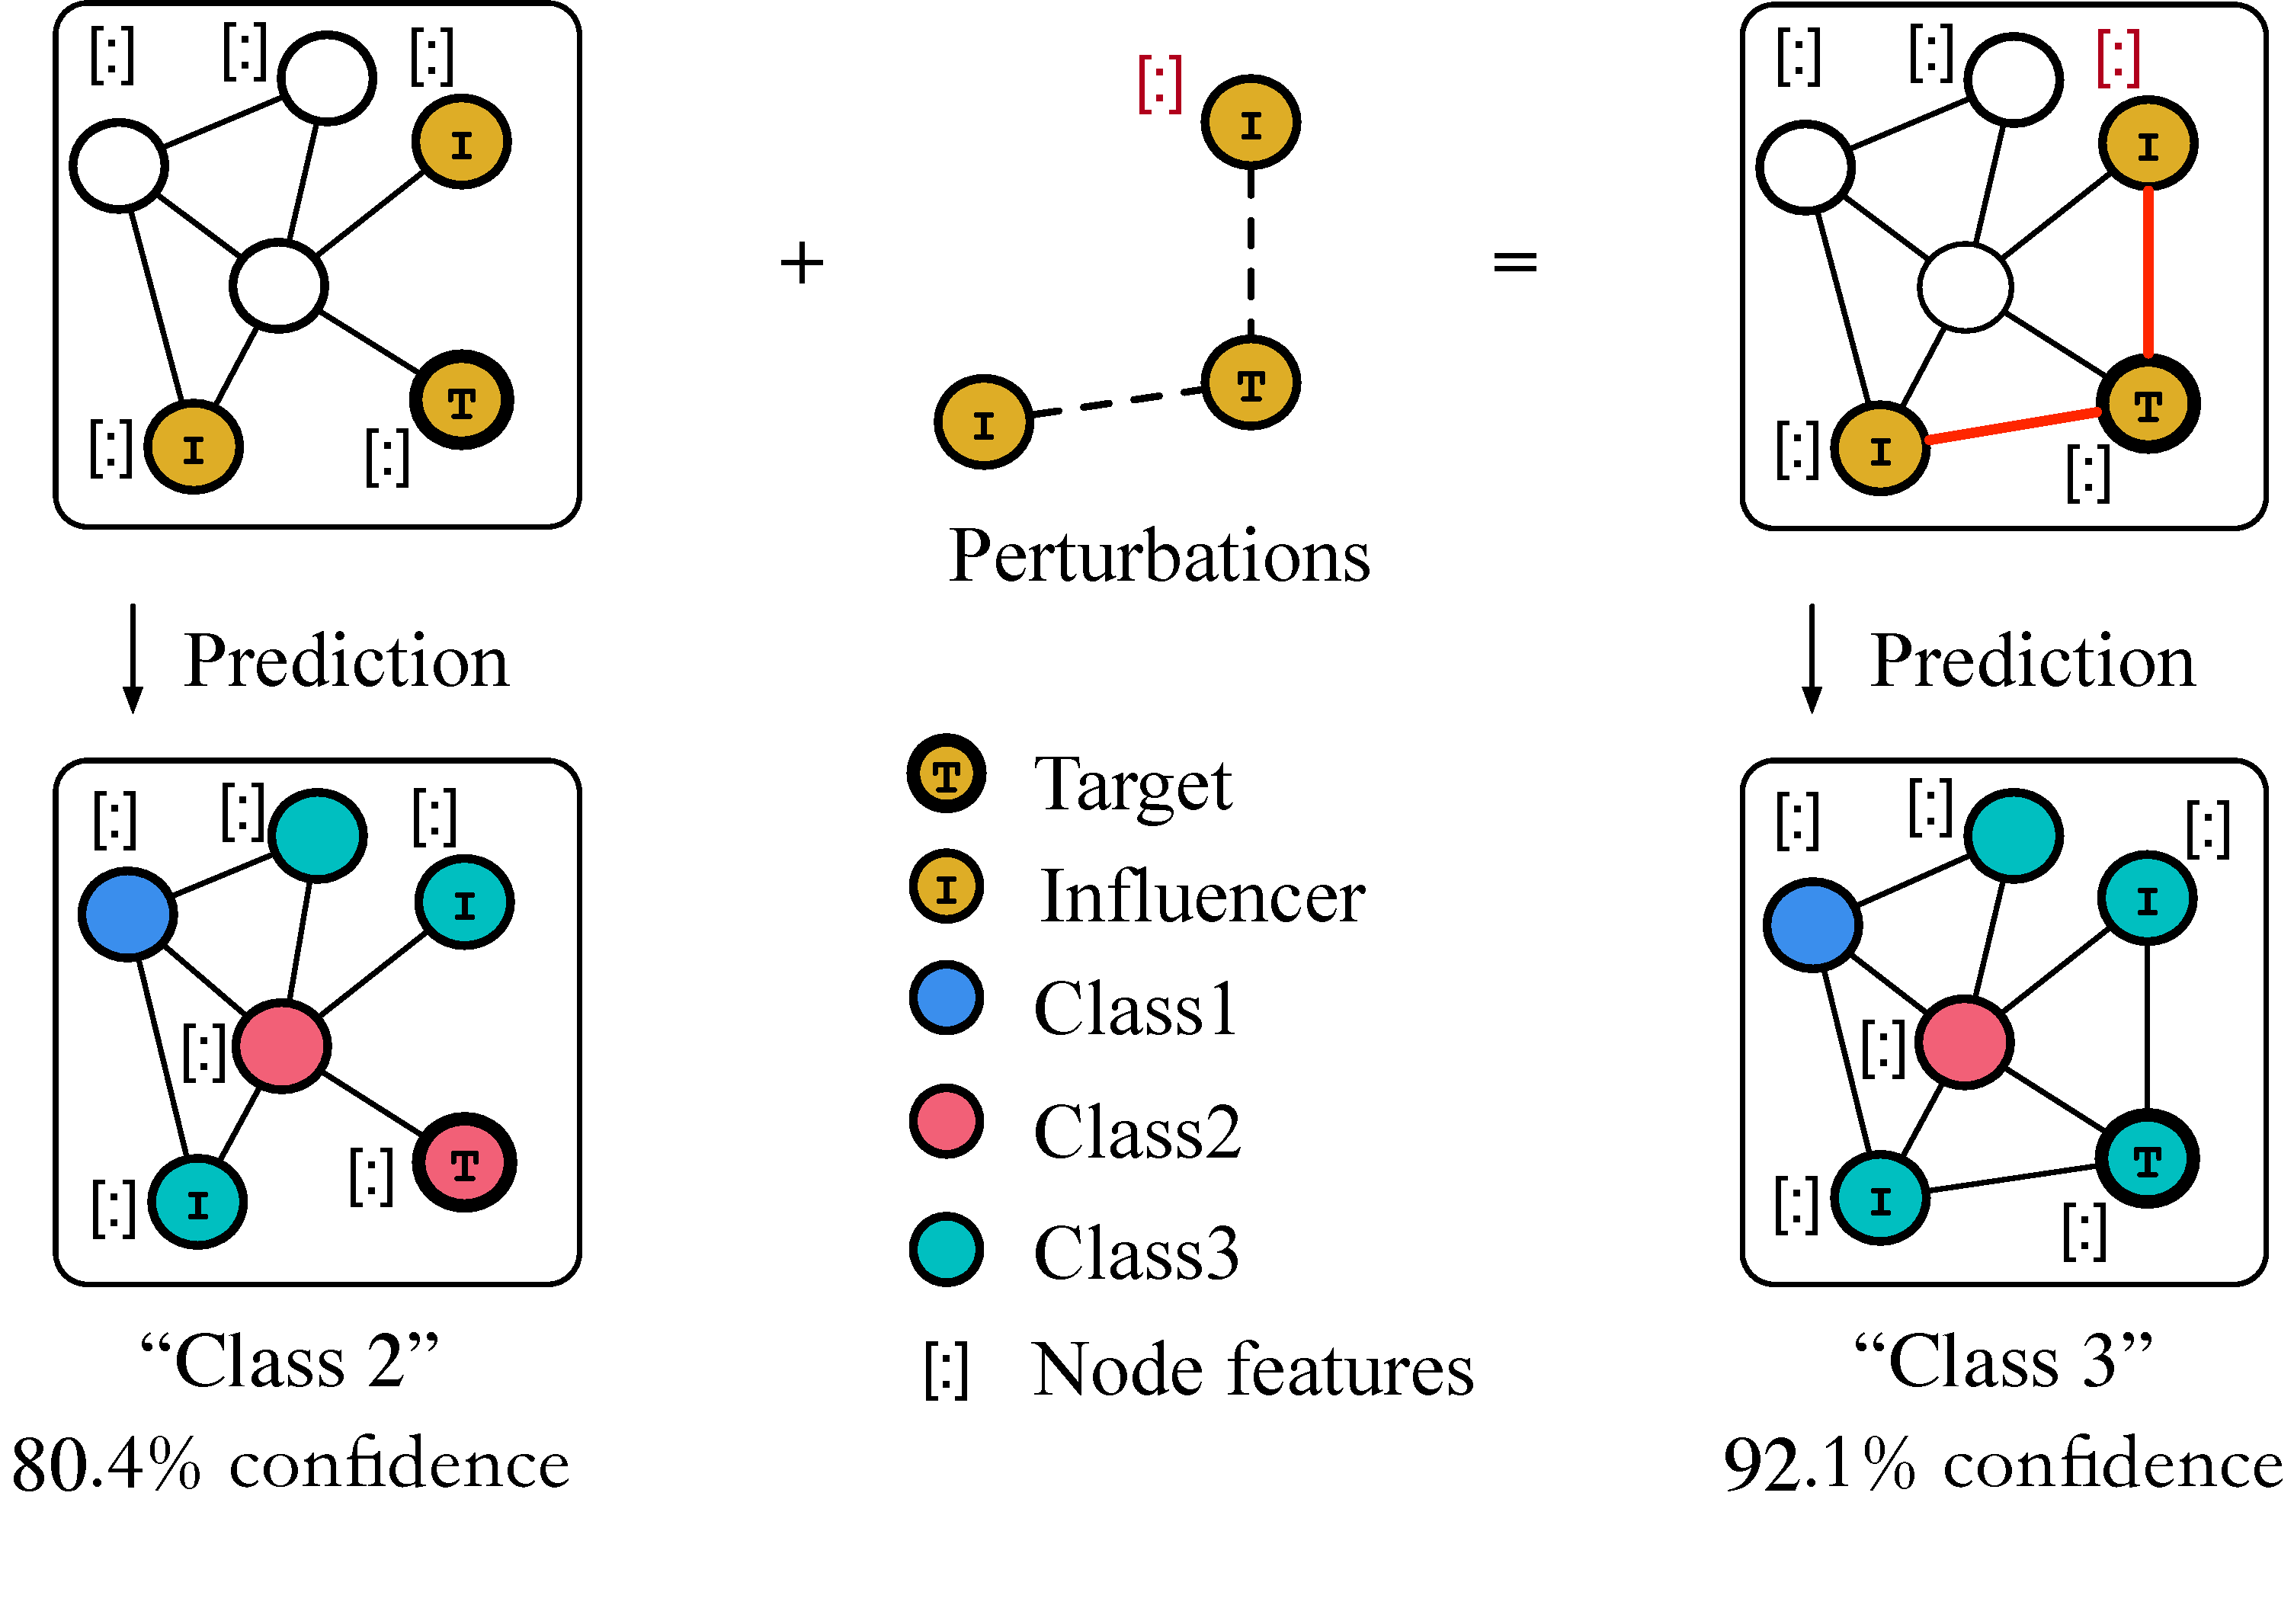
\includegraphics[width=\linewidth]{AttackDiagram.pdf}\\
	\caption{A misclassification of the target caused by a small perturbations of the graph structure and node features.}
	\label{Fig1}
\end{figure}

With rising concerns being paid on the security of graph models, there exists a surge of researches on graph adversarial learning, i.e., a field on studying the security and vulnerability of graph models. On one hand, from the perspective of attacking a graph learning model, Z\"ugner et al. \cite{zugner2018adversarial} first study adversarial attacks on graph data, with little perturbations on node features and graph structure, the target classifiers are easily fooled and misclassify specified nodes. On the other hand, Wang et al. \cite{wang2019adversarial} propose a modified Graph Convolution Networks (GCNs) model with an adversarial defense framework to improve its robustness. Moreover, Sun et al. \cite{sun2018adversarial} study the existing works of adversarial attack and defense strategies on graph data and discuss their corresponding contributions and limitations. However, they mainly focus on the aspect of the adversarial attack, leaving works on defense unexplored.

\nosection{Challenges} Despite a surge of works on the graph adversarial learning, there still exists several problems to solve. i) \emph{Unified and specified formulation}. Current studies consider the problem definition and assumptions in graph adversarial learning with their own mathematical formulations and mostly lack of detailed explanations, which effectively hinders the progress of follow-up studies. ii) \emph{Related evaluation metrics}. While for various tasks, evaluation metrics on corresponding performance are rather different, and even have diverse standardization on it. Besides, special metrics for the graph adversarial learning scenario are necessary and timely to explore, e.g., evaluation on the attack impacts.

% 第一个是针对定义不统一，我们所做的工作。
For the problem of inconsistent formulations and definitions, we survey the existing attack and defense works, give unified definitions and categorize them from diverse perspectives. Although there have been some efforts \cite{zugner2018adversarial,ma2019attacking,dai2018adversarial} to generalize the definitions, most formulations still make customization for their own models. So far, only one article \cite{sun2018adversarial} outlines these concepts from a review perspective, which is not sufficient to summarize the existing works comprehensively. Based on the previous literature, we summarize the different types of graphs and introduce the three main tasks according to the level, and subsequently give the unified formulations of attack and defense in Section \ref{attackDefinition} and \ref{defenseDefinition}, respectively.

Different models have various metrics due to different emphasis. To provide guidance for researchers and better evaluate their adversarial models, we have a more detailed summarize and discussion on metrics in Section \ref{metrics}. In particular, we first introduce some common metrics for both attack and defense, and then present some special metrics provided in their respective works from three categories: effectiveness, efficiency, and imperceptibility. For instance, the Attack Success Rate (ASR) \cite{chen2018link} and the Average Defense Rate (ADR) \cite{chen2019can} are proposed to measure the effectiveness of attack and defense, respectively.

In summary, our contributions can be listed as bellow:
\begin{itemize}
	\item We thoroughly investigate related works in this area, and subsequently give the unified problem formulations and the clear definitions for current inconsistent concepts of both attack and defense.
	\item We give a clear overview on existing works and classify them from different perspectives based on reasonable criteria systematically.
	\item We emphasize the importance of evaluation metrics and investigate them to make a comprehensively summary.
	      %		\item We point out the potential valuable research directions in the future study.
	\item For such an emerging research area, we point out the limitations of current researches and provide some open questions to solve.

\end{itemize}
The survey is organized as follow. In Section \ref{preliminary}, we will give some basic notations of typical graphs. In Section \ref{attack} and Section \ref{defense}, we will separately introduce the definitions, taxonomies of adversarial attack and defense on graph data, and further give a clear overview. We then summarize the related metrics in Section \ref{metrics} and try to discuss some open research questions in Section \ref{openProblems}. Finally, we draw our conclusion in Section \ref{conclusion}.

\begin{table*}[t]
	\centering
	\caption{Summary of notations.}
	\label{notation_table}
	\scalebox{0.8}{
		\begin{tabular}{c|c||c|c||c|c}
			\hline
			\hline
			Symbol                     &
			Description                &
			Symbol                     &
			Description                &
			Symbol                     &
			Description                  \\

			\hline
			\begin{tabular}[c]{@{}c@{}} $N$ \end{tabular}  &
			\begin{tabular}[c]{@{}c@{}} number of nodes \end{tabular}  &
			\begin{tabular}[c]{@{}c@{}} \\ $M$\\ \\ \end{tabular}  &
			\begin{tabular}[c]{@{}c@{}} number of edges \end{tabular}  &
			\begin{tabular}[c]{@{}c@{}} \\ $n$\\ \\ \end{tabular}  &
			\begin{tabular}[c]{@{}c@{}} number of graphs \end{tabular}
			\\

			\hline
			\begin{tabular}[c]{@{}c@{}} $F_{(\cdot)}$ \end{tabular} &
			\begin{tabular}[c]{@{}c@{}} number of features w.r.t. \\
				nodes $F_{(node)}$ or edges $F_{(edge)}$\end{tabular} &
			\begin{tabular}[c]{@{}c@{}} \\ $\tilde{G}$\\ \\ \end{tabular} &
			\begin{tabular}[c]{@{}c@{}} a graph instance, denoting \\
				a clean graph $G$ or a modified graph $\hat{G}$\end{tabular} &
			\begin{tabular}[c]{@{}c@{}} \\ $\mathcal{C}$\\ \\ \end{tabular} &
			\begin{tabular}[c]{@{}c@{}} set of pre-defined class labels \\ for nodes, edges or graphs \end{tabular}
			\\

			\hline
			\begin{tabular}[c]{@{}c@{}} \\ $\mathcal{V}$\\ \\ \end{tabular} &
			\begin{tabular}[c]{@{}c@{}} set of nodes $\mathcal{V}=\{v_1,v_2,\dots,v_N\}$ \end{tabular} &
			\begin{tabular}[c]{@{}c@{}} $\mathcal{E}$ \end{tabular} &
			\begin{tabular}[c]{@{}c@{}} set of edges $\mathcal{E}=\{e_1,e_2,\dots,e_M\}$ \end{tabular} &
			\begin{tabular}[c]{@{}c@{}} $\mathcal{G}$ \end{tabular} &
			\begin{tabular}[c]{@{}c@{}} set of graphs $\mathcal{G}=\{G_1,G_2,\dots,G_n\}$ \end{tabular}
			\\

			\hline
			\begin{tabular}[c]{@{}c@{}} $\mathcal{D}$ \end{tabular} &
			\begin{tabular}[c]{@{}c@{}} the whole dataset,\\ $\mathcal{D}=(\mathcal{G}, X, \mathcal{C})$ \end{tabular} &
			\begin{tabular}[c]{@{}c@{}} \\ $\mathcal{S}$\\ \\ \end{tabular} &
			\begin{tabular}[c]{@{}c@{}} set of instances, could be $\mathcal{G}$, $\mathcal{V}$, or $\mathcal{E}$ \end{tabular} &
			\begin{tabular}[c]{@{}c@{}} $\mathcal{S}_L$ \end{tabular} &
			\begin{tabular}[c]{@{}c@{}}  set of labeled instances, could be\\ $\mathcal{G}_L$, $\mathcal{V}_L$, or $\mathcal{E}_L$,  $S_L \subset S$ \end{tabular}
			\\

			\hline
			\begin{tabular}[c]{@{}c@{}} \\ $\mathcal{T}$\\ \\ \end{tabular} &
			\begin{tabular}[c]{@{}c@{}} set of unlabeled instances\\ where $\mathcal{T} \subset \mathcal{S}-\mathcal{S}_L$ or $\mathcal{T} = \mathcal{S}-\mathcal{S}_L$ \end{tabular} &
			\begin{tabular}[c]{@{}c@{}} \\ $\mathcal{K}$\\ \\ \end{tabular} &
			\begin{tabular}[c]{@{}c@{}}attackers' knowledge of the dataset \end{tabular} &
			\begin{tabular}[c]{@{}c@{}} \\ $\mathcal{O}$\\ \\ \end{tabular} &
			\begin{tabular}[c]{@{}c@{}}operation set\\ w.r.t. attackers' manipulation \end{tabular}
			\\



			\hline

			\begin{tabular}[c]{@{}c@{}}  $A$ \end{tabular} &
			\begin{tabular}[c]{@{}c@{}} adjacency matrix $A \in \mathbb{R}^{N\times N}$ \end{tabular} &
			\begin{tabular}[c]{@{}c@{}} \\ $A'$\\ \\ \end{tabular} &
			\begin{tabular}[c]{@{}c@{}} modified adjacency matrix \end{tabular} &
			\begin{tabular}[c]{@{}c@{}} $X$ \end{tabular} &
			\begin{tabular}[c]{@{}c@{}} feature matrix\\ $X \in \{0,1\}^{N \times F_{(\cdot)}}$ or $X \in \mathbb{R}^{N \times F_{(\cdot)}}$ \end{tabular}

			\\

			\hline

			\begin{tabular}[c]{@{}c@{}} \\ $X'$\\ \\ \end{tabular} &
			\begin{tabular}[c]{@{}c@{}} modified feature matrix \end{tabular} &
			\begin{tabular}[c]{@{}c@{}} $f$ \end{tabular} &
			\begin{tabular}[c]{@{}c@{}} deep learning model w.r.t. inductive \\ learning  $f^{(ind)}$ or transductive learning $f^{(tra)}$\end{tabular} &
			\begin{tabular}[c]{@{}c@{}} \\ $\hat{f}$\\ \\ \end{tabular} &
			\begin{tabular}[c]{@{}c@{}} surrogate model \end{tabular}

			\\

			\hline

			\begin{tabular}[c]{@{}c@{}} $\tilde{f}$ \end{tabular} &
			\begin{tabular}[c]{@{}c@{}} well-designed model for defense \end{tabular} &
			\begin{tabular}[c]{@{}c@{}} \\ $\theta$\\ \\ \end{tabular} &
			\begin{tabular}[c]{@{}c@{}} set of parameters\\ w.r.t. a specific model \end{tabular} &
			\begin{tabular}[c]{@{}c@{}} $Z$ \end{tabular} &
			\begin{tabular}[c]{@{}c@{}} output of the model \end{tabular}

			\\

			\hline
			\begin{tabular}[c]{@{}c@{}} \\ $t$\\ \\ \end{tabular} &
			\begin{tabular}[c]{@{}c@{}} target instance,\\ can be a node, an edge or a graph \end{tabular} &
			\begin{tabular}[c]{@{}c@{}} $\Delta$ \end{tabular} &
			\begin{tabular}[c]{@{}c@{}} attack budgets \end{tabular} &
			\begin{tabular}[c]{@{}c@{}} \\ $y$\\ \\ \end{tabular} &
			\begin{tabular}[c]{@{}c@{}} ground-truth label\\ w.r.t. an instance, $y \in \mathcal{C}$ \end{tabular}

			\\

			\hline
			\begin{tabular}[c]{@{}c@{}} \\ $\Psi$\\ \\ \end{tabular} &
			\begin{tabular}[c]{@{}c@{}} perturbation space \\of attacks \end{tabular} &
			\begin{tabular}[c]{@{}c@{}} \\ $\mathcal{L}$\\ \\ \end{tabular} &
			\begin{tabular}[c]{@{}c@{}} loss function of \\deep learning model \end{tabular} &
			\begin{tabular}[c]{@{}c@{}} \\ $\mathcal{Q}$\\ \\ \end{tabular} &
			\begin{tabular}[c]{@{}c@{}} similarity function \\of graphs\end{tabular}
			\\

			\hline
			\hline
		\end{tabular}
	}
\end{table*}


\section{Preliminary}
\label{preliminary}

Focusing on the graph structure data, we first give notations of typical graphs for simplicity and further introduce the mainstream tasks in graph analysis fields. The most frequently used symbols are summarized in Table \ref{notation_table}.
\subsection{Notations}
\label{notation}
Generally, a graph is represented as $\mathcal{G}=(\mathcal{V},\mathcal{E})$, where $\mathcal{V}=\{v_1, v_2, \dots, v_N \}$ denotes the set of $N$ nodes and $\mathcal{E}=\{e_1, e_2, \dots, e_M \}$ is the set of $M$ existing edges in the graph, and naturally $\mathcal{E} \subseteq \mathcal{V} \times \mathcal{V}$. The connections of the graph could be represented as an adjacency matrix $A \in \mathbb{R}^{N\times N}$, where $A_{i,j}\neq 0$ if there is an edge from node $v_i$ to node $v_j$ and $A_{i,j}=0$ otherwise.

% 	\begin{figure}[h] 
%         \centering 
%         \includegraphics[width=80mm]{Resources/Preliminary.pdf}\\ 
%         \caption{Heterogeneous graph (a) and dynamic graph (b). (a) Different types of nodes denote as different colors.} 
%         \label{Fig2}
%     \end{figure}

\subsection{Taxonomies of Graphs}
Different scenarios correspond to various types of graphs, hence we will introduce them further in the following parts based on the basic graph definition in Section \ref{notation}.

\nosection{\textbf{Directed and Undirected Graph}} Directed graph, also called a digraph or a directed network, is a graph where all the edges are directed from one node to another  — but not backwards \cite{chartrand1977introductory}. On the contrary, a graph where the edges are bidirectional is called an undirected graph. For undirected graphs, the convention for denoting the adjacency matrix doesn't matter, as all edges are bidirectional. Generally, $A_{i,j}\neq A_{j,i}$ for directed graph and $A_{i,j}=A_{j,i}$ for undirected graph.

\nosection {\textbf{Weighted and Unweighted Graph}} Typically a weighted graph refers to an edge-weighted graph where each edge is associated with a real value \cite{chartrand1977introductory}. An unweighted graph may be used if a relationship in terms of magnitude doesn’t exist, i.e., the connections between edges are treated as the same.

\nosection {\textbf{Attributed Graph}}
An attributed graph refers to a graph where both node and edge are available to have its own attributes/features \cite{ding2019deep}. Specifically, the attributes of nodes and edges could be denoted as $X_{node} \in \mathbb{R}^{N\times F_{node}}$ and $X_{edge} \in \mathbb{R}^{M \times F_{edge}}$, respectively. In most cases a graph usually have attributes associated with nodes only, we use $X$ to denote the node attributes/features for brevity.

\nosection {\textbf{Homogeneous and Heterogeneous Information Graph}}
As well as attributes, the type of nodes or edges is another important property. A graph $\mathcal{G}$ is called heterogeneous information graph if there are two or more types of objects/nodes or relations/edges in it \cite{liu2018heterogeneous,hussein2018meta}; otherwise, it is called a homogeneous information graph.

\nosection {\textbf{Dynamic and Static Graph}}
Intuitively, nodes, edges and attributes are possibly changing over time in a dynamic graph \cite{manessi2020dynamic}, which could be represented at $\mathcal{G}^{(t)}$ at time $t$. For a static graph, which is simply defined as $\mathcal{G}$, in which nodes, edges and attributes remain the same as the time changes.

Each type of graph has different strengths and weaknesses. It's better to pick the appropriate kind of graph to model the problem. As existing works are mainly focus on a simple graph, i.e., undirected and unweighted. Besides, they assume that the graph is static and homogeneous for simplicity. By default, the mentioned ``graph'' refers to ``simple graph'' in this paper.

\subsection{Graph Analysis Tasks}
\label{task}
In this section, we will introduce the major tasks of graph analysis, in which deep learning models are commonly applied to. From the perspective of nodes, edges and graphs, we divide these tasks into three categories: node-, link- and graph-level task.

\nosection{\textbf{Node-level Task}}
Node classification is one of the most common node-level tasks, for instance, identifying a person in a social network. Given a graph $\mathcal{G}$, with partial labeled nodes $\mathcal{V}_L \subseteq \mathcal{V}$ and other unlabeled ones, the goal of classifiers is to learn a mapping function $\phi: \mathcal{V} \rightarrow \mathcal{C}$, where $\mathcal{C}$ is a set of pre-defined class labels. The learned mapping function is applied to effectively identify the class labels for the unlabeled nodes \cite{kipf2017semi}. To this end, inductive learning and transductive learning settings are specified based on the characteristic of training and testing procedures.
\begin{itemize}
	\item \emph{Inductive Setting}. For the inductive learning setting, a classifier is usually trained on a set of nodes and tested on others that never seen during training.
	\item \emph{Transductive Setting}. Different from inductive setting, test samples (i.e., the unlabeled nodes)  can be seen (but not their labels!) during the training procedure in transductive learning setting.
\end{itemize}
To conclude, the objective function that optimized by the classifier could be formulated as follows:
\begin{equation}
	\label{loss}
	\mathfrak{L}= \frac{1}{|\mathcal{V}_L|} \sum_{v_i \in \mathcal{V}_L}\mathcal{L}(f_{\theta} (\mathcal{G}, X), y_i)
\end{equation}
where $y_i$ is the class label of node $v_i$, and $\mathcal{L}$ could be the loss of either inductive learning or transductive learning, and the classifier $f$ with parameters $\theta$ is similarly defined with the two settings.


\nosection{\textbf{Link-level Task}}
Link-level task relates to the edge classification and link prediction. Among them, link prediction is a more challenging task and widely used in real-world, which aims to predict the connection strength of an edge, e.g., predicting the potential relationship between two specified persons in a social network, and even the new or dissolution relationship in the future. Link prediction tasks take the same input as node classification tasks, while the output is binary which indicates an edge will exist or not. Therefore the objective function of link prediction tasks could be similarly defined as Eq.(\ref{loss}) by changing $y_i \in \{0,1\}$, and replacing $\mathcal{V}_L$ with a set of labeled edges $\mathcal{E}_L$.


\nosection{\textbf{Graph-level Task}}
While treating the graph as a special form of node, the graph-level tasks are similar to node-level tasks. Take the most frequent application, graph classification, as an example, the graph $\mathcal{G}$ could be represented as $\mathcal{G}=\{ G_1, G_2,\dots, G_n \}$, where $G_i=(\mathcal{V}_i,\mathcal{E}_i)$ is a subgraph of the entire graph. The core idea to solve the graph classification problem is to learn a mapping function $\mathcal{G} \rightarrow \mathcal{C}$, here $\mathcal{C}$ represents the set of graph categories, so as to predict the class for an unseen graph more accurately. The objective function of graph classification tasks is similar with Eq.(\ref{loss}) as well, in which the labeled training set is $\mathcal{G}_L$ instead of $\mathcal{V}_L$, and $y_i$ is the category of the graph $G_i$. In real world, graph classification task plays an important role in many crucial applications, such as social and biological graph classification.